% An weighted directed graph

\documentclass[]{standalone}

\usepackage{tikz}

\begin{document}

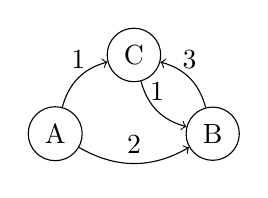
\begin{tikzpicture}

	% Nodes circled

	\node[draw, circle, minimum size=0.5cm] (A) at (0, 0) {A};
	\node[draw, circle, minimum size=0.5cm] (B) at (2, 0) {B};
	\node[draw, circle, minimum size=0.5cm] (C) at (1, 1) {C};

	% Curved edges
	% \draw[->] (A) to [bend right] (B);
	% \draw[->] (A) to [bend left] (C);
	% \draw[->] (B) to [bend right] (C);
	% \draw[->] (C) to [bend right] (B);

	% Edges with weights
	\draw[->] (A) to [bend right] node[above] {2} (B);
	\draw[->] (A) to [bend left] node[above] {1} (C);
	\draw[->] (B) to [bend right] node[above] {3} (C);
	\draw[->] (C) to [bend right] node[above] {1} (B);
\end{tikzpicture}

\end{document}